
\section{Object specification}
\label{sec:objects}


Generally speaking the code will be organized around roughly three object type categories involved in the structure of the new HOPS. These are as follows:

\begin{enumerate}
 \item Meta Data Containers: These serve to store small quantities of station and baseline metadata associated with an observation of disparate types.
 \item Array Containers: These serve to organize large n-dimensional arrays of a single data type (e.g. visibility data and correction/calibration table data).
 \item Data Operators: These evaluate a function or perform some transformation on a given data container. Their operation is configurable via a set of externally defined parameters, while their application to any particular data set can be made conditional by a set of filters.).
\end{enumerate}

\subsection{Data Containers}

The existing HOPS3 code base relies on a fixed number of \texttt{C} structs to organize and present the data related to an observation. The strict memory layout of these structures has the advantage of making them cross-machine compatible, which is necessary since these structures are also used as the core components of the Mark-4 I/O library. However, a notable disadvantage of this rigid design is the degree of difficulty encountered in making changes to the existing data structures, or adding new data types in order to accommodate additional information which was not originally envisioned at the time the library was written. To make the data structures more flexible we intend to decouple the in-memory data layout from the file I/O, so they do not necessarily need to be byte-for-byte copies.

\subsubsection{Meta-Data Containers}

In a strictly typed language such as \texttt{C}, flexible data structures have a high degree of code overhead, not only in the management of dynamic memory allocation, but more severely in the conversion of data types and typecasting. To ameliorate this we propose to exploit \texttt{C++11}'s variadic template mechanism, which allows for the transformation of type-agnostic class lists into concrete class types or hierarchies at compile time. This makes it possible to store disparate types (so long as the complete set of types is known at compile time) within in the same object that are indexed and can be retrieved by the same type of key (e.g. a name string). Listing~\ref{lst:metaobjects} gives a condensed example of the preliminary version of the template base class for a meta-data container (with detailed functionality removed).

\lstinputlisting[language=C++,float=h!,label={lst:metaobjects},caption=Meta-data object template classes for multi-type maps.]{code/metadata-objects.hh}

To the extent possible, the in-memory meta-data structures should be classes which provide access via a key-value pair mechanism so as to avoid exposing the private internal storage layout to the routines needing access to subsets of the data. This retrieval mechanism also has the benefit of completely decoupling the compile
time structure of the data containers from the data they need to hold at runtime. A key:value interface is trivially available via the STL std::map template class,
so there is no need to expend effort on a native implementation. Moreover this sort of interface should also make conversion of these data structures into widely accessible formats such as JSON or python dictionaries possible for data export to external software.

\subsubsection{N-Dimensional Array Containers}

We propose the following basic set of class templates be used to construct most in-memory objects used for the manipulation of correlated observation data and its associated station data:
\begin{enumerate}
 \item \texttt{MHO\_ScalarContainer} - encapsulates scalar-like data
 \item \texttt{MHO\_VectorContainer} - encapsulates vector-like data
 \item \texttt{MHO\_TableContainer} - encapsulates rank-N tensor-like data with associated axes (vector)
\end{enumerate}
These template classes are to serve as a simple wrapper around the management of the raw memory needed to store a data item and keep track of its associated unit(s), and (if applicable) the values associated with the axes along each dimension and their units.

The three container types listed above represent the majority of the memory intensive data needed within HOPS
and can largely be derived from a N-dimensional array of some numeric or integral type. Therefore a generic template class for
N-dimensional arrays is needed, listing \ref{lst:ndarray} shows a stub of this class.
\lstinputlisting[language=C++,label={lst:ndarray},caption=N-Dimensional Array Template]{code/MHO_NDArrayWrapper.hh}
The underlying storage of the N-dimensional array data is done as a single contiguous chunk of memory which can either be a piece of externally or internally managed memory. Indexing into this chunk of memory is done using C-like row-major order, where for an array of rank D, with dimension sizes $\{N_0, N_1, \cdots N_{D-1}\}$, the location of the data specified by the indexes $\{n_0, n_1, \cdots, n_{D-1}\}$ can found at an offset from the start, $z$, that is given by:
\begin{equation}
 z = \sum_{k=0}^{D-1} \left ( \prod_{j=k+1}^{D-1} N_j \right) n_k
 \end{equation}
Access to the underlying data stored within a class of this type can then proceed in two main ways. The first is through the aforementioned
row-major order indexing operation, and the second is through the use of iterators. An example of several of the provided methods is shown for a three dimensional array in listing \ref{lst:array-usage}. Iterators are most commonly utilized for efficient incremental (continuous or strided) access to the array data as they can be computed using pointer arithmetic, while random access is best done via indexes.
\lstinputlisting[language=C++,label={lst:array-usage},caption=N-Dimensional Array access]{code/array_use.cc}

In addition to the raw data stored in the N-dimensional array, in the case of the \texttt{MHO\_TableContainer} it is important to associate a coordinate axis with each dimension in order to provide various data operators with the ability to look-up the location of a datum beyond a simple integer-index. To enable this,
we will pair an N-dimensional array with a tuple of axis objects associated with each dimension. Listing \ref{lst:objects} shows the template class structure
for a TableContainer (along with other) objects.
\lstinputlisting[language=C++,float=h!,label={lst:objects},caption=Data object templates]{code/data-objects.hh}
The axis objects themselves also inherit from \texttt{MHO\_IntervalLabelTree}, which provides the ability to associate a pair of indexes with a key value pair of several types. A simple example of this would be tagging a section of the frequency axis with a particular channel ID (e.g \texttt{ [0, 32] } $\leftrightarrow$ \texttt{ \{"channel\_id": "X17LY"\} }). The class \texttt{MHO\_IntervalLabelTree} will support tagging axis intervals with values of at least the following types: char, bool, int, double, and string, using strings as keys, and allow for the bi-directional look up of a key:value pairs with assoiated intervals.

As a concrete example of the \texttt{MHO\_TableContainer} template class, listing \ref{lst:visib} gives a simple example of what template declaration of an object storing channelized visibility data from a single-baseline observation might look like.
\lstinputlisting[language=C++,float=h!,label={lst:visib},caption=Visibility object type]{code/visibilities.hh}
For example, in the case of channelized visibilities, the axes of each of the four dimensions would be:
\begin{enumerate}
\item Axis 0: Polarization-product axis, labelled by a short string specifying the reference
and remote stations' polarizations for data associated with that column (e.g ``XX'' or ``RR'' or ``RX'').
\item Axis 1: Channel axis, labelled by a character or numerical value (e.g. ``A'' or 1).
\item Axis 2: Time axis, labelled by the time since start of a scan in seconds.
\item Axis 3: Frequency axis, labelled by the frequency offset from the edge of the channel (MHz).
\end{enumerate}
It should be noted that these coordinate axes are there merely to label the data, but are not meant to provide a reverse look-up
capability, (e.g example inverting the polarization-product code ``LL'' to infer a 0-th index location of 0). For efficiency array
access should still be done using unsigned integer index values. A graphical representation of a \texttt{MHO\_TableContainer} is
shown in Figure~\ref{fig:table-container}.

\begin{figure}[h!]
  \begin{center}
  \captionsetup{width=0.7\linewidth}
  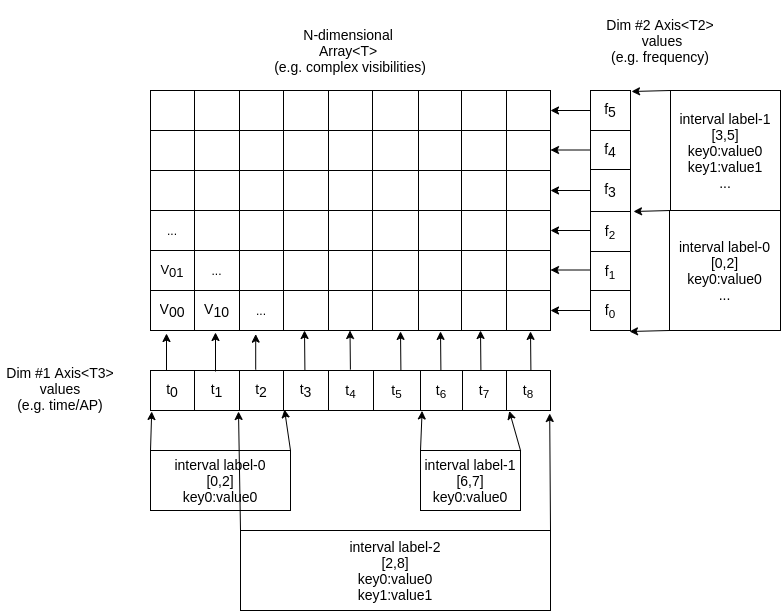
\includegraphics[width=0.75\textwidth]{fig/data-container-baseline.png}
    \caption{A graphical representation of a \texttt{MHO\_TableContainer}. This class is composed of an N-dimensional array, coupled with axes to provide coordinate values along each dimension. The axes themselves allow for arbitrary intervals to be labelled by key:value pairs in order to allow for local look-up of filter data. For example, along the frequency axis, the interval labels may be channel or sampler names among other possibilities. Furthermore, the interval and associated labels will be stored in an interval-tree structure to allow for fast bi-directional lookup of data indices $\leftrightarrow$ data labels.}
    \label{fig:table-container}
\end{center}
\end{figure}

\subsubsection{Specific data types}

Below is an incomplete table of the various data objects that are constructed from \texttt{MHO\_TableContainer}, along with their data value type and axis names.
\begin{center}
\resizebox{\textwidth}{!}{
\begin{tabular}{| c | c | c | c |}
\hline
 Name & value type & N-Dim & Axes \\  \hline
 Visibilities & \texttt{std::complex<double>} & 3 & (pol. product, time, frequency) \\ \hline
 Weights & \texttt{double} & 3 & (pol. product, time, frequency) \\ \hline
 Flags & \texttt{uint64\_t} & 3 & (pol. product, time, frequency) \\ \hline
 Channelized Visibilities & \texttt{std::complex<double>} & 4 & (pol. product, channel, time, frequency) \\ \hline
 Channelized Weights & \texttt{double} & 4 & (pol. product, channel, time, frequency) \\ \hline
 Channelized Flags & \texttt{uint64\_t} & 4 & (pol. product, channel, time, frequency) \\ \hline
 (static) per-Channel phase corrections & \texttt{double} & 2 & (pol. product, channel) \\ \hline
 Channelized Ad-hoc phases/amplitude corrections  & \texttt{std::complex<double>} & 4 & (pol. product, channel, time, frequency) \\ \hline
 \end{tabular}
 }
\end{center}

\subsection{Data operators}

The data operator classes are meant to organize the mathematic manipulations which are to be performed on the data containers. For example, many of the operations performed in the existing HOPS3 code-base (such as the application of a priori phase calibration) are relatively trivial linear transformations applied to the visibility data. However, they are currently intertwined with a large amount of control logic which obscures the basic data pathway (e.g see postproc/fourfit/norm\_fx.c)

Most unary or binary operations that are to applied to visibility or other data residing in an \texttt{HO\_TableContainers} such as scaling, multiplication, transposition, summation, Fourier transformation, etc. will be made available as individual classes inheriting from the same interface. A uniform class interface will allow these data operators to be composed or modified to create more complicated composite operators or strung together and called in an ordered fashion in order to accomplish data pipelines of arbitrary complexity. An additional advantage of encapsulating individual operations is that (coupled with the data container extensions) any SIMD parallel-processing extension used to accelerate data processing can be made opaque to the user.

Listing \ref{lst:operators} gives a brief sketch of the class templates generalizing the data operators. The common inheritance from the base class \texttt{MHO\_Operator} allows them all to be stored in an common container (e.g. \texttt{std::vector<MHO\_Operator*>}) so that once they are
constructed and configured they may be retrieved and intialized/executed in the appropriate order. Listing \ref{lst:operator-use} shows a brief code
sketch demonstrating how two simple operators would be constructed, assigned arguments and then initialized and executed in order.

\lstinputlisting[language=C++,float=h!,label={lst:operators},caption=Data operator template classes.]{code/operator_use.cc}

It is expected that the vast majority of the data operators will be unary or binary, requiring only their own configuration parameters along with one or two data containers upon which they operate as inputs. 
However, any number of arguments is possible so long as the underlying implementation provides the appropriate overload.

One aspect of the data operators which is not yet detailed here is a notion of what pieces of meta-data each operator may need in order to complete its function. 
Some of the more primitive operations (e.g. complex conjugation) may not need any meta-data, while certain 
specific calibration routines may need station related meta-data (e.g. channel specific phase-cal).
While some meta-data items could be exposed directly via external setter/getters, a possibly preferable option which would preserve encapsulation might be for each operator to define an internal schema, 
listing the keys and type of the parameters it needs to retrieve from a single meta-data container (populated from the vex), or what sort of labels it expects to be attached to the data containers on which it operates.
In addition, a mechanism for filtering operations (e.g. if station = Xx, then apply this operator) also needs to be established independent of the previous control-block structure of HOPS3.

\lstinputlisting[language=C++,float=h!,label={lst:operators},caption=Data operator template classes.]{code/data-operators.hh}

\subsubsection{Specific data operations}

Below is an incomplete list of various data operations. A full specification of each operation is detailed in the subsequent pages.
\begin{enumerate}
 \item MHO\_ComplexConjugator: Apply a complex conjugation to all elements of an ND-array.
 \item MHO\_CyclicRotator: Apply a cyclic rotation to the selected axes of an ND-array.
 \item MHO\_FastFourierTransform: Apply a Fourier transform to a one dimensional array.
 \item MHO\_FunctorBroadcaster: Apply a specified unary function to each element of an ND-array.
 \item MHO\_MultidimensionalFastFourierTransform: Apply a Fourier transform to the selected axes of an ND-array using native libary.
 \item MHO\_MultidimensionalFastFourierTransformFFTW: Apply a Fourier transform to the selected axes of an ND-array using FFTW library.
 \item MHO\_MultidimensionalPaddedFastFourierTransform: Apply a zero-padded Fourier transform to the selected axes of an ND-array.
 \item MHO\_Reducer: Apply a reduction (e.g. sum all elements) along the selected axis of an ND-array.
 \item MHO\_SubSample: Skip select every n-th element of an ND-array for a specified axis of a ND-array.
\end{enumerate}

\newpage

\noindent \textbf{Name:} MHO\_ComplexConjugator \\
\textbf{Type:} Unary, in-place and out-of-place (requires copy). \\
\textbf{Configuration Parameters:} None\\
\textbf{Inputs:} An N dimensional array with complex double/float value type \\
\textbf{Outputs:} An N dimensional array with complex double/float value type \\
\textbf{Description:} Iterates over all values in an N dimensional array and applies the operation \texttt{std::conj()} to each element. \\

\newpage 

\noindent \textbf{Name:} MHO\_CyclicRotator \\
\textbf{Type:} Unary, both in-place and out-of-place. \\
\textbf{Configuration Parameters:} Requires the integer index of the axis to be rotated, and the integer offset specifying the size of the rotation.\\
\textbf{Inputs:} An N dimensional array with any primitive type \\
\textbf{Outputs:} An N dimensional array with any primitive type \\
\textbf{Description:} \\

\newpage 

\noindent \textbf{Name:} MHO\_FastFourierTransform \\
\textbf{Type:} Unary, both in-place and out-of-place. \\
\textbf{Configuration Parameters:} None\\
\textbf{Inputs:} A one dimensional array with complex double/float value type \\
\textbf{Outputs:} A one dimensional array with complex double/float value type \\
\textbf{Description:} \\


\newpage 

\noindent \textbf{Name:}  MHO\_FunctorBroadcaster \\
\textbf{Type:} Unary, both in-place and out-of-place. \\
\textbf{Configuration Parameters:} \\
\textbf{Inputs:} \\
\textbf{Outputs:} \\
\textbf{Description:} \\


\newpage 

\noindent \textbf{Name:} MHO\_MultidimensionalFastFourierTransform \\
\textbf{Type:} Unary, both in-place and out-of-place. \\
\textbf{Configuration Parameters:} None\\
\textbf{Inputs:} An N dimensional array with complex double/float value type \\
\textbf{Outputs:} An N dimensional array with complex double/float value type \\
\textbf{Description:} \\

\newpage 

\noindent \textbf{Name:} MHO\_MultidimensionalFastFourierTransformFFTW \\
\textbf{Type:} Unary, both in-place and out-of-place. \\
\textbf{Configuration Parameters:} None\\
\textbf{Inputs:} An N dimensional array with complex double/float value type \\
\textbf{Outputs:} An N dimensional array with complex double/float value type \\
\textbf{Description:} \\

\newpage 

\noindent \textbf{Name:} MHO\_MultidimensionalPaddedFastFourierTransform \\
\textbf{Type:} Unary, both in-place and out-of-place. \\
\textbf{Configuration Parameters:} None\\
\textbf{Inputs:} An N dimensional array with complex double/float value type \\
\textbf{Outputs:} An N dimensional array with complex double/float value type \\
\textbf{Description:} \\


\newpage 

\noindent \textbf{Name:} MHO\_Reducer  \\
\textbf{Type:} Unary, both in-place (requires copy and resize) and out-of-place. \\
\textbf{Configuration Parameters:} \\
\textbf{Inputs:} \\
\textbf{Outputs:} \\
\textbf{Description:} \\

\newpage 

\noindent \textbf{Name:} MHO\_SubSample  \\
\textbf{Type:} Unary, both in-place and out-of-place. \\
\textbf{Configuration Parameters:} \\
\textbf{Inputs:} \\
\textbf{Outputs:} \\
\textbf{Description:} \\




\subsubsection{Data Container Extensions}

The primary goal of the containers is to provide a relatively simple and efficient representation of commonly used data types that hides the details of
memory management and array indexing/access from the user. They should not be overburdened with too much extraneous functionality that is specific to a particular operation that must be executed upon them (e.g. the N-dimensional array container should not implement a method to sum two arrays.), as this greatly
over complicates these classes and makes them brittle. However, there are some cases where this sort of decoupling may induce a performance cost. An example of
this occurs in the case of SIMD/GPU acceleration. In order to make use of GPU processing the data must be copied to a buffer on the device, processed, and then the results must be passed back to the host. However, if there are several operations to be performed in succession on the GPU, only first and last transfer
need to occur, with intervening transfers being unecessary as input data is already present on the device. However, in order to eliminate the intermediate transfers a handle to the device buffer must be kept available. While a pointer a device buffer does not belong in something as basic as a data container, it
is a good candidate for something to be stored in and extension.

In order to provide the ability to append extensions to the data containers, they must all inherit from a base class, \texttt{MHO\_ExtensbleElement}, which
in turn stores a vector of type-erased\footnote{https://davekilian.com/cpp-type-erasure.html} pointers to the extensions themselves. The extensions are templated on the the class providing the additional functionality and must all inherit from the base class \texttt{MHO\_ExtendedElement} (so they can be stored in the vector owned \texttt{MHO\_ExtensbleElement}) A brief sketch of the code that allows for this is shown in listing \ref{lst:extend}. One draw back of this method is that it requires $N$ \texttt{dynamic\_cast} calls (where $N$ is the number of extensions) every time any particular extension is modified or accessed via the data container. This is an acceptable trade off for infrequent access to expensive (to construct) extensions, but should be used rather sparingly as \texttt{dynamic\_cast} has high overhead.

\lstinputlisting[language=C++,float=h!,label={lst:extend},caption=Data container extension classes.]{code/MHO_ExtensibleElement.hh}
